\documentclass[12pt,a4paper]{article}
\renewcommand{\thesection}{\Roman{section}}
\renewcommand{\thesubsection}{\thesection.\Roman{subsection}}
\usepackage{xeCJK}
\usepackage{caption}
\usepackage{amssymb}
\usepackage{amsmath}
\usepackage{geometry}
\usepackage{subfigure}
\usepackage{fancyhdr}
\usepackage[export]{adjustbox}
\usepackage{graphicx}
\graphicspath{{images/}}
\geometry{left=2.5cm,right=1.5cm,top=2cm,bottom=2cm}
\begin{document}
\begin{enumerate}
  \item First, since we don't have wheel odometry, the parameter \textbf{"odom\_used" is set to false}. Second, since we only have visual odometry with topic name /zed/odom instead of vo, it has to \textbf{remap from vo to /zed/odom} to make the node work properly.
  \item IMU provides orientation information (called function \textbf{tf::quaternionMsgToTF}) while not position information since it is not reliable after double integration from acceleration. For visual odometry, it provides both position and orientation (called function \textbf{tf::poseMsgToTF}) since it offers relatively reliable position information by visual cues.
  \item The figure that illustrated 7 settings is shown in Fig. \ref{fig:com}. Since we don't have the groundtruth, we can only qualitative describe the result. Since only visual odometry provides positional information, no matter how we change the magnitude of position variance, the filtered path will not affected.%if we shrink the position variance for VO, the filtered path will more close to original one (notice the curve when it turned right). The similar behavior occurs in orientation of VO. In fourth row, there is not significant differences between two settings, I guess it is because we only visualize the position but not orientation.
If we shrink the variance of orientation from VO, the filtered path will approach to original one (as 3rd row). For IMU, if we enlarge the variance of it, the path will mroe similiar with the original one.  
To answer the problem that which setting is better, we must understand the strengths of each sensors and setup our system correctly (transformation between sensors and robot, etc.). In this dataset, if we make IMU variance even smaller, the path will incline to the left which is incorrect apparently, so I may more believe the data from visual odometry.
  
\begin{figure}[hbt]
  \centering
  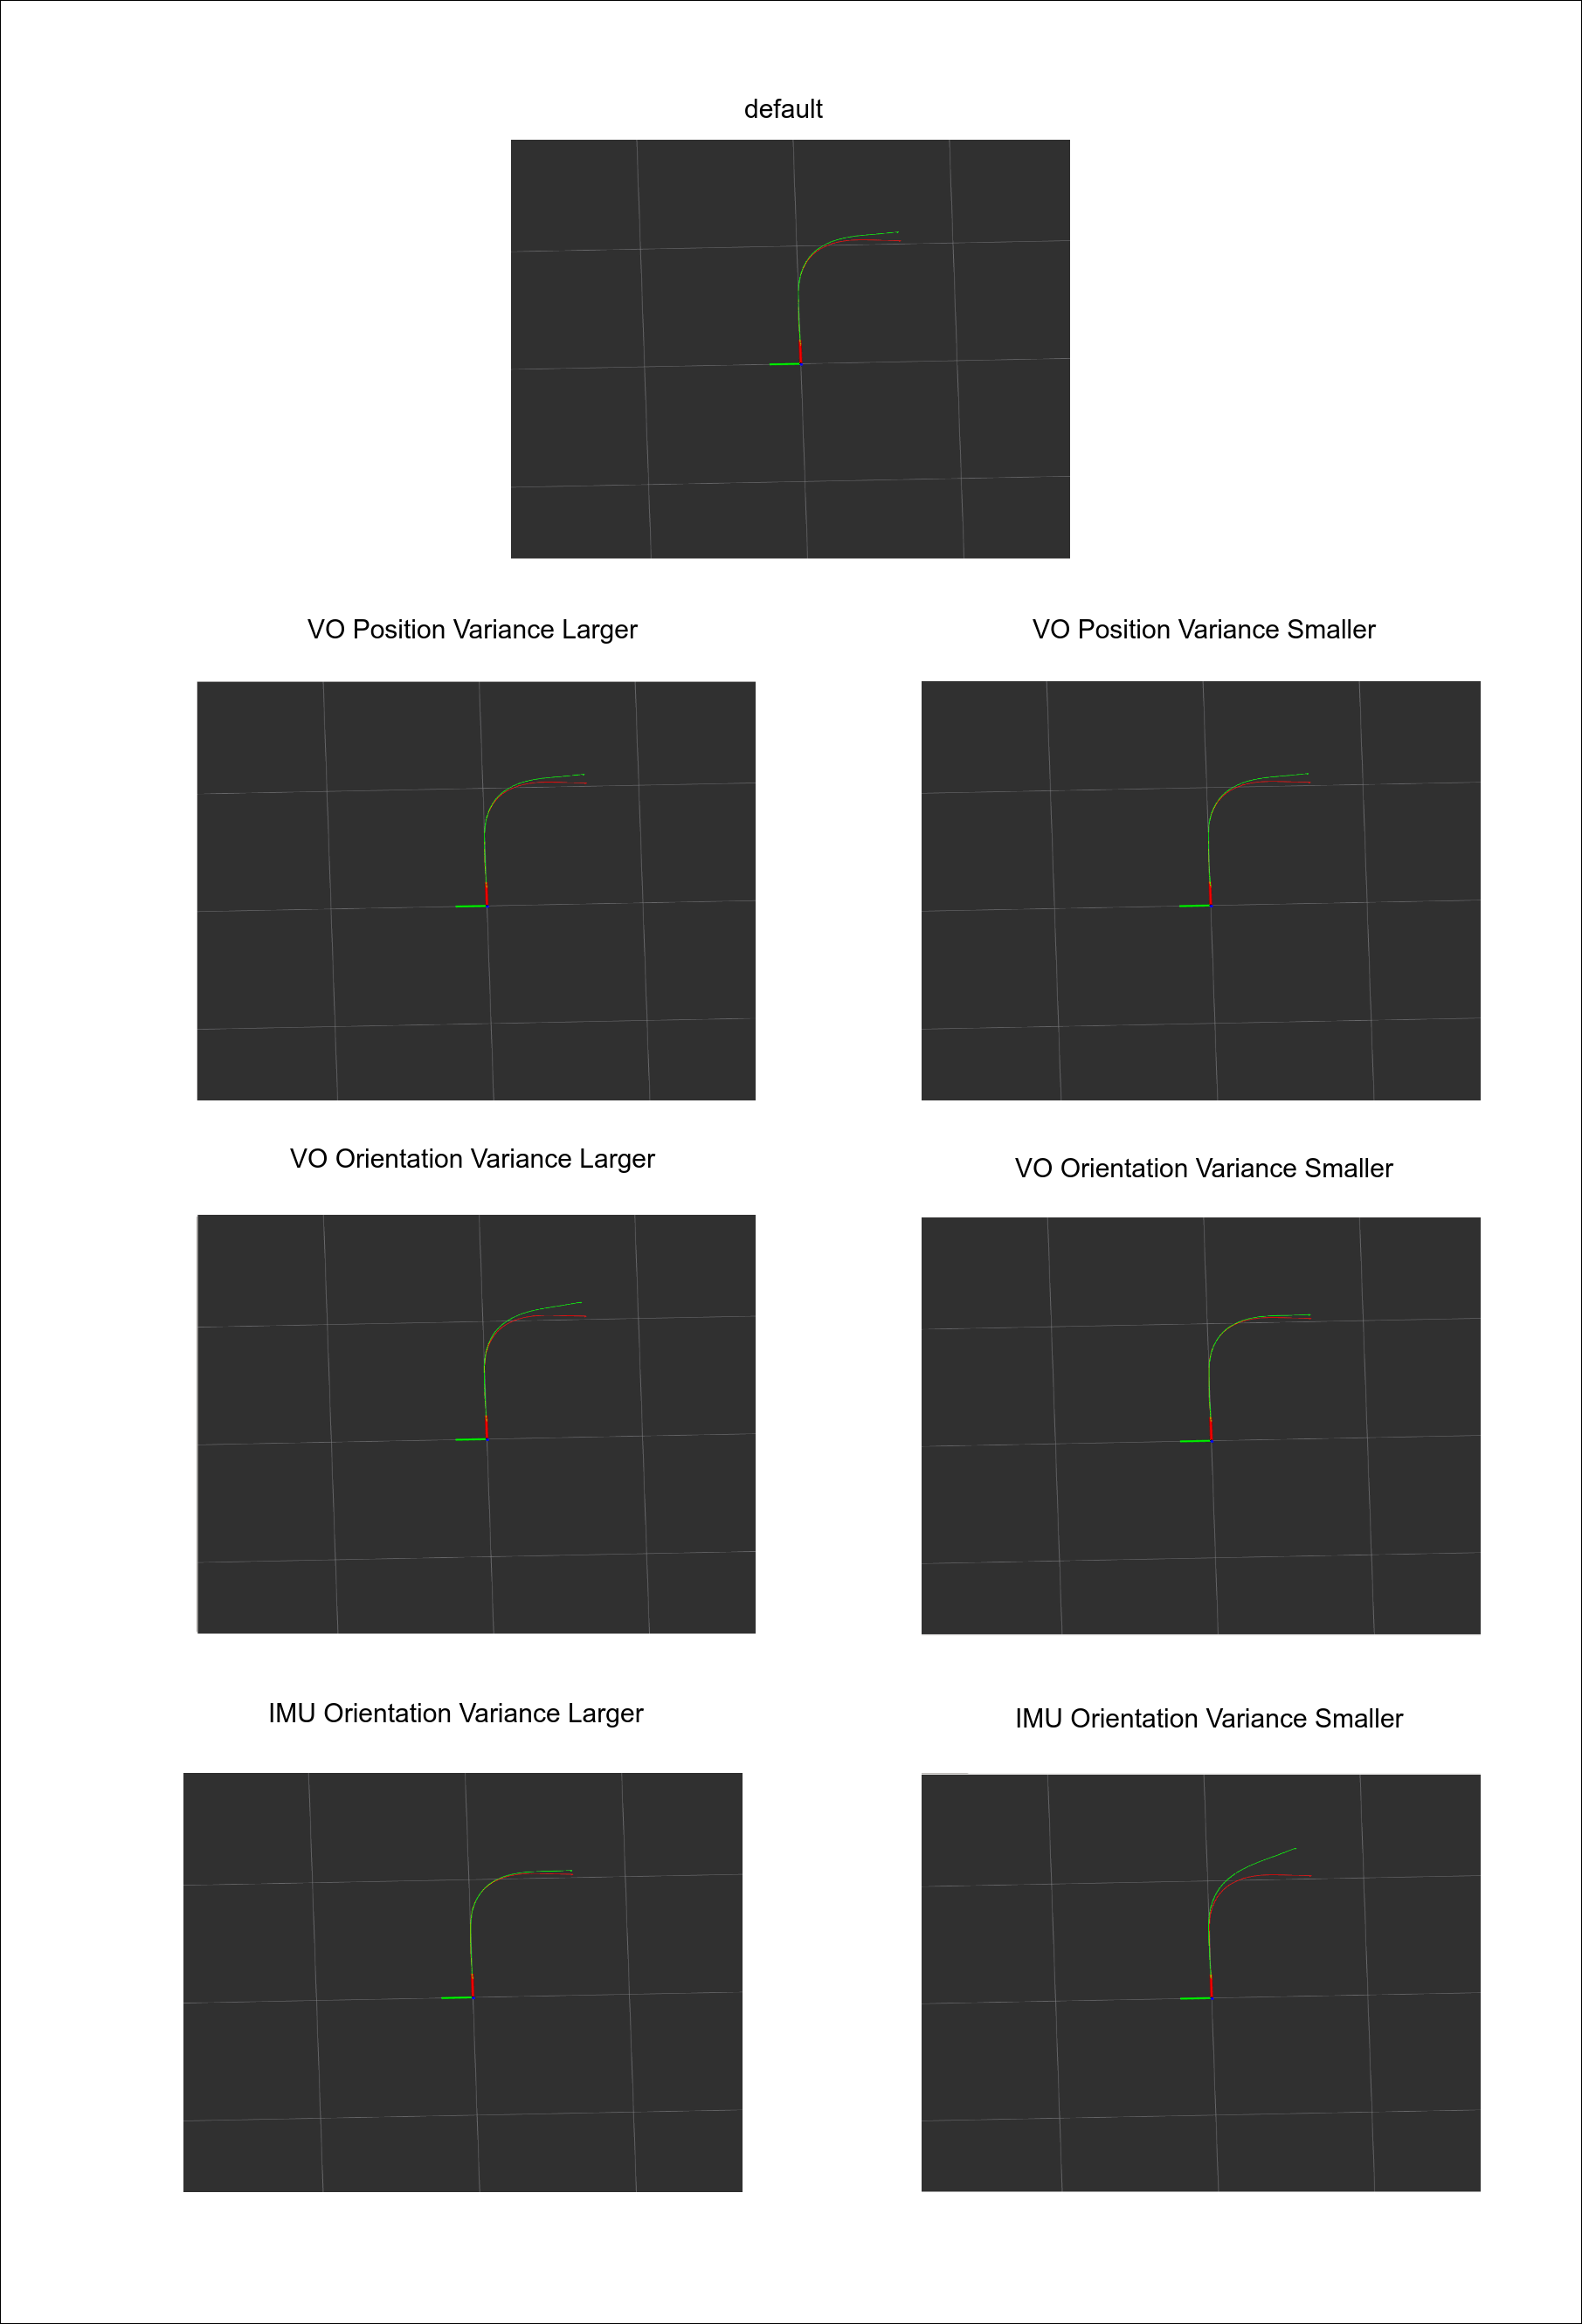
\includegraphics[scale=0.27]{combined.png}
  \caption{Comparision Between 7 Settings}
  \label{fig:com}
\end{figure}
\end{enumerate}
\end{document}
